\documentclass[10pt]{article}
\usepackage[letterpaper,margin=0.7in]{geometry}
\usepackage{graphicx}
\usepackage{float}
\setlength{\intextsep}{5pt}
\usepackage[hidelinks]{hyperref}
\graphicspath{{figures/}}
\renewcommand{\thefigure}{S\arabic{figure}}
\begin{document}
\begin{center}
{\Large Supplementary Figures}\\[5pt]
Morphology-Aware Rolling Whole-Body Planning for\\
Aerial Continuum Manipulation in Confined Spaces
\end{center}
Supplementary Fig.~S1 reports attitude and load diagnostics from three PX4/Gazebo runs. Figures~S2 and S3 show the original visual--strain records and their evaluation references.

\begin{figure}[H]
\centering
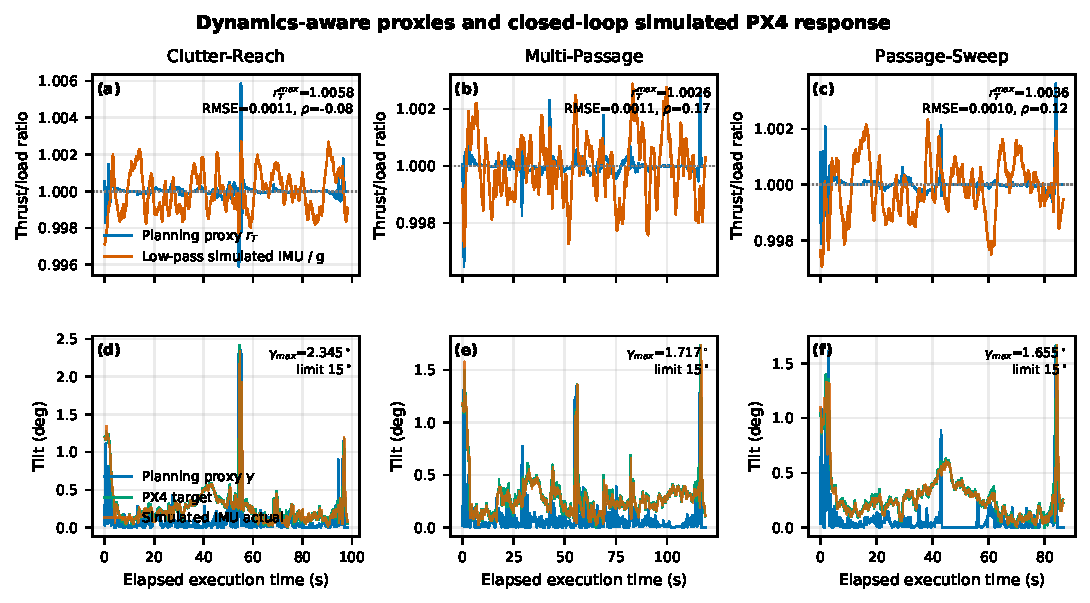
\includegraphics[width=0.94\textwidth]{fig08_dynamics_proxy_validation.pdf}
\caption{Supplied flight-response and load-proxy comparison. Realized-versus-PX4-target tilt statistics describe attitude tracking. Normalized IMU specific-force magnitude is an indirect load-related quantity, not a direct measurement of individual rotor thrust. The low-dynamic traces do not validate a complete rigid--soft coupled dynamics model.}
\end{figure}
\clearpage
\begin{figure}[H]
\centering
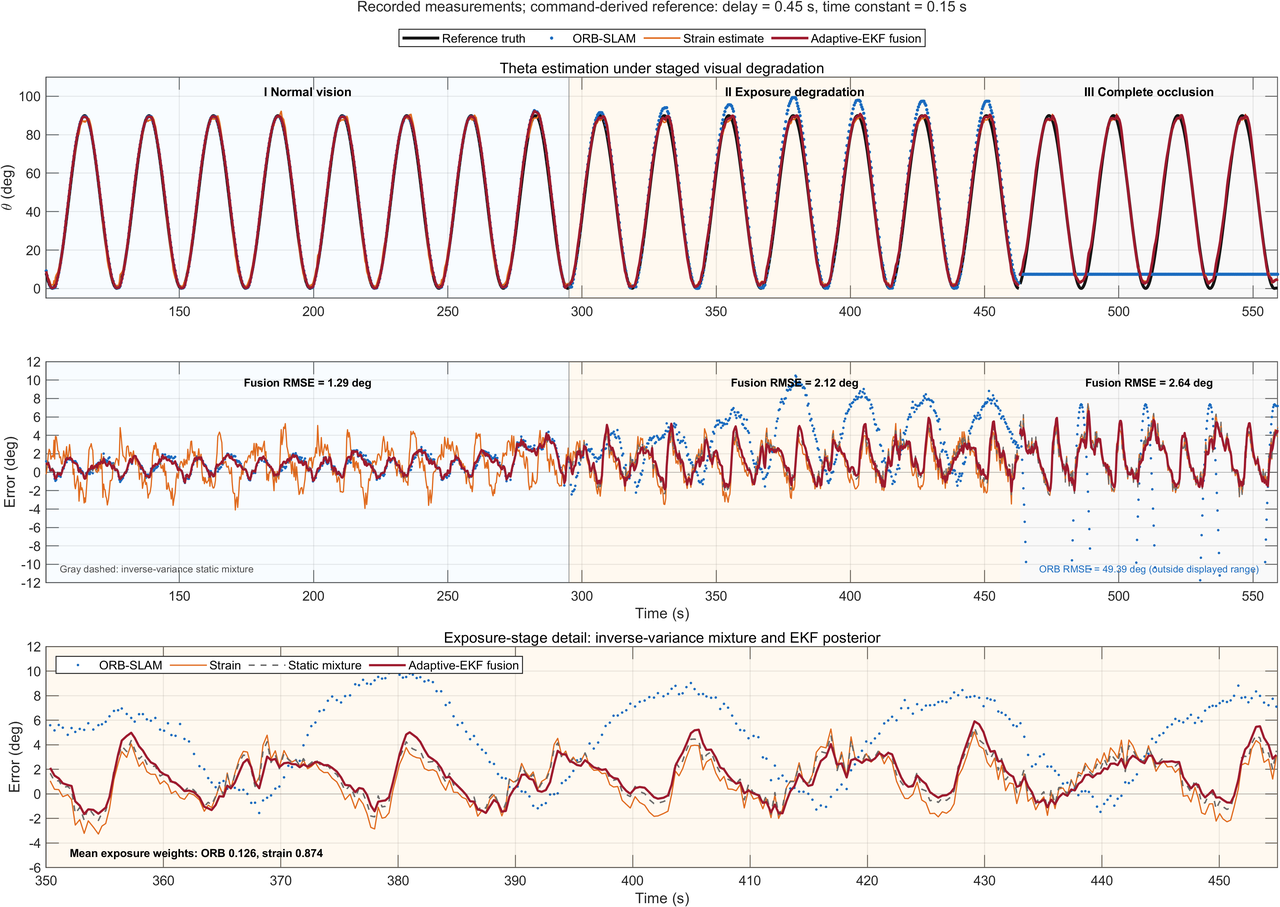
\includegraphics[width=0.87\textwidth,height=8.1in,keepaspectratio]{fig_sensor_theta_fusion.png}
\caption{Original bending-magnitude record, including angle trajectories, fusion weights, residuals, and printed statistics. The supplied asset labels its reference as command-derived. The displayed residual range is narrower than the full ORB error after tracking loss; no missing residual samples have been reconstructed. Consequently, visual residual amplitudes alone should not be used to compare failure-stage accuracy. The original complete asset is retained for traceability.}
\end{figure}
\clearpage
\begin{figure}[H]
\centering
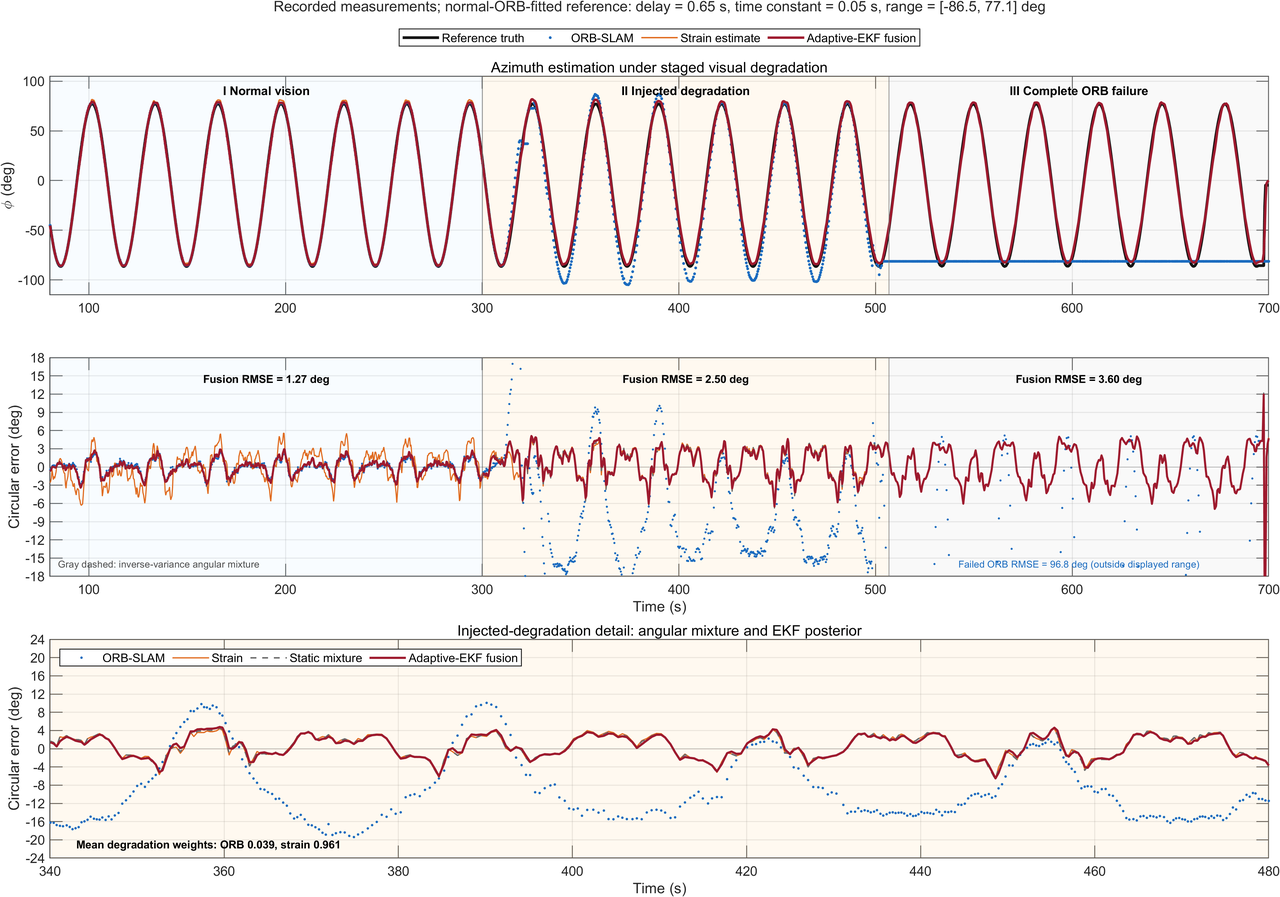
\includegraphics[width=0.87\textwidth,height=8.1in,keepaspectratio]{fig_sensor_phi_fusion.png}
\caption{Original bending-plane record. The supplied reference was fitted from normal ORB observations, as indicated in the source image. Its failure-stage residual plot has a limited display range, while the full angle traces show the frozen visual estimate. The reference and residual limits preclude interpreting the printed errors as independent motion-capture test accuracy. All original panels and annotations are preserved.}
\end{figure}
\end{document}
